\section{Introduction}
\begin{frame}{Attitude Estimation}

Attitude estimation is the process of estimating the orientation of an aerospace vehicle with respect to an intertial frame of reference. \\~\\

Usually, in navigation, attitude is estimated with 3 angles:
\begin{itemize}
\item \textbf{Yaw}: angle respect to true north. Heading.
\item \textbf{Pitch}: angle of the nose respect to the horizon. Angle of attack.
\item \textbf{Roll}: angle of the wings respect to the horizon. Bank.
\end{itemize}

\begin{center}
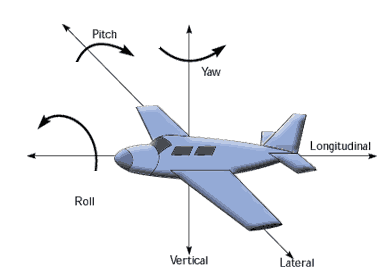
\includegraphics[width=0.5\textwidth]{figures/attitude.png}
\end{center}
\end{frame}


\begin{frame}{Sensors}
To perform attitude estimation, sensors are needed:
\begin{itemize}
\item Accelerometer: gives direction of gravity.
\item Gyroscope: gives rate of turn.
\item Magnetometer: gives direction of magnetic north.
\end{itemize}
\end{frame}